\documentclass[11pt]{article}
\usepackage[margin=1in]{geometry}
\usepackage{amsmath,amssymb,amsthm,mathtools}
\usepackage{dsfont}
\usepackage{graphicx}
\usepackage{booktabs}
\usepackage{array}
\usepackage{placeins}
\usepackage[hyphens]{url}
\usepackage{microtype}
\usepackage{xcolor}
\usepackage{tikz}
\usepackage{caption}
\usepackage{subcaption}
\captionsetup{singlelinecheck=off}
\usepackage[colorlinks=true,linkcolor=blue!55!black,citecolor=blue!55!black,urlcolor=blue!55!black]{hyperref}

\newcommand{\Tr}{\operatorname{Tr}}
\newcommand{\tr}{\operatorname{tr}}
\newcommand{\Var}{\operatorname{Var}}
\newcommand{\Np}{N'}
\newcommand{\one}{\mathds 1}
\newcommand{\End}{\operatorname{End}}
\newcommand{\Ad}{\operatorname{Ad}}
\newcommand{\lib}{\mathrm{lib}}
\newcommand{\OU}{\mathrm{OU}}
\newcommand{\dec}{\mathrm{dec}}

% status tags (as in the 29 September report)
\definecolor{cest}{RGB}{30,90,160}
\definecolor{cder}{RGB}{20,120,70}
\definecolor{cnum}{RGB}{150,90,10}
\definecolor{cconj}{RGB}{160,40,40}
\newcommand{\tagbox}[2]{\textsf{\small\color{#1}[#2]}}
\newcommand{\EST}{\tagbox{cest}{literature}}
\newcommand{\DER}{\tagbox{cder}{derived}}
\newcommand{\VER}{\tagbox{cder}{derived + verified}}
\newcommand{\NUM}{\tagbox{cnum}{numerical}}
\newcommand{\CONJ}{\tagbox{cconj}{conjecture}}
\newcommand{\INTERP}{\tagbox{cconj}{interpretation}}

% chord-diagram palette (as in the 29 September report)
\definecolor{cP}{HTML}{2A78D6}   % P arcs
\definecolor{cPp}{HTML}{EB6834}  % P' / P_x arcs
\definecolor{cX}{HTML}{8E2C8A}   % chords joining the two kinds
\definecolor{cM}{HTML}{555555}   % random matter / H arcs
\tikzset{
  Parc/.style={line width=3.4pt, cP},
  Pparc/.style={line width=3.4pt, cPp},
  Harc/.style={line width=3.4pt, cM!45},
  chP/.style={line width=1.0pt, cP!85!black},
  chPp/.style={line width=1.0pt, cPp!90!black},
  chH/.style={line width=1.0pt, cM},
  chX/.style={line width=1.15pt, cX, dash pattern=on 3.2pt off 1.8pt},
  chM/.style={line width=1.6pt, black, dash pattern=on 4pt off 2pt},
  Umark/.style={draw=black, fill=white, rectangle, inner sep=1.8pt, line width=0.8pt},
  Mmark/.style={draw=black, fill=black, circle, inner sep=1.6pt},
}
\newcommand{\chord}[4][]{\draw[#1] ({#2}:{#4}) .. controls ({#2}:{0.32*#4}) and ({#3}:{0.32*#4}) .. ({#3}:{#4});}
\newcommand{\Umk}[2]{\node[Umark] at ({#1}:{#2}) {};}
\newcommand{\Mmk}[2]{\node[Mmark] at ({#1}:{#2}) {};}

\newtheorem{proposition}{Proposition}
\theoremstyle{remark}
\newtheorem*{remark}{Remark}

\title{\bf Progress report, 5 October 2026:\\ chord number is chaos degree,\\ and the decoder's fourth moment
is\\ free liberation plus localization}
\author{\texttt{syk\_gravity} project\\[2pt]\small Drafted by Claude for J.~Chryssanthacopoulos; code state: commit
\texttt{4395248} (branch \texttt{t4-fourarc})}
\date{}

\emergencystretch=2em
\renewcommand{\topfraction}{0.92}
\renewcommand{\bottomfraction}{0.6}
\renewcommand{\textfraction}{0.06}
\renewcommand{\floatpagefraction}{0.8}
\begin{document}
\maketitle

\begin{abstract}
\noindent
The 29 September report~\cite{prog0929} closed with three ``next computations'' (its \S7.3). This report answers the
first and most of the second. Throughout, $P$ is the BPS projector of one-flavor $\mathcal N{=}2$ SYK ($p=3$), the decoder is
$O=P(1-n_i)P$, and $P'=UPU$ with $U=(-1)^{n_i}$.
\begin{itemize}\itemsep1pt
\item \textbf{Chord number is a Wiener-chaos degree} (item 7.3.1). For OU-correlated couplings
  $\omega_x=x\omega+\sqrt{1-x^2}\,\omega'$, one has exactly $E\,\tau(P(\omega)P(\omega_x))=\sum_n\pi_nx^{2n}$, with $\pi_n$
  the weight of the $n$-th chaos of $P$. This is BLY's chord-number distribution with exact finite-$N$ weights. Size is
  bounded by chord number, $k\le(p-1)n$ at half filling (plethysm). The chord-1 sector is exactly $\gamma H^{(2)}$, with
  a closed form that tends to BLY in double scaling.
\item \textbf{One generating function for decoder and OU pairs} (item 7.3.2). The decoder, the isotropic OU family and a
  ``site-local'' family are evaluations of one Mehler series at different coupling correlations.
\item \textbf{Isotropic deformations look free.} Along the whole OU family, $T_4$ as a function of $T_2$ is within
  $\le0.012$ of \emph{free liberation} (a free unitary Brownian rotation of $P$, which has a closed form). The deviation
  tracks the known two-model non-freeness.
\item \textbf{The decoder is local.} At equal $T_2$ the decoder exceeds the OU curve by $0.017$--$0.047$ in $T_4$.
  Gaussian resampling of only the couplings touching site $i$ reproduces two thirds of this, and the same family's
  $\mathbb Z_2$ endpoint reproduces it exactly.
\item \textbf{What $R$ is.} The decoder's excess over the Wachter value splits as 68--78\,\% free liberation (analytic),
  $\le5\,\%$ isotropic non-freeness and 37\,$\to$\,19\,\% localization ($\Np=8\to14$). The remainder $R$ of the 29 September
  decomposition is a small difference between a negative liberation piece and a positive localization piece.
\end{itemize}
Consequence for a gravity computation: the universal object is the isotropic four-arc function, an overlap of two
mismatched BPS wormholes. The localization piece is a finite-$p$, site-level effect that structureless matter chords
cannot capture. Tags: \EST, \DER, \VER, \NUM, \INTERP, \CONJ.
\end{abstract}

\tableofcontents

%=====================================================================
\section{Summary of results}
%=====================================================================
\begin{enumerate}\itemsep3pt
\item \VER\ \textbf{Chord number = chaos degree} (\S\ref{sec:chaos}).
  $E\,\tau(P(\omega)P(\omega_x))=\sum_n\pi_nx^{2n}$, with $\pi_n=E\|P_{[n]}\|^2/d$ and $\pi_0=a$ exactly. In the chord
  expansion each Wick contraction across the cut carries $x$. In double scaling this is the second quantization
  $x^{\hat N}$ of Bożejko--Kümmerer--Speicher, applied to SYK by Pluma--Speicher \EST.
\item \VER\ \textbf{Selection rule} (\S\ref{sec:selection}). The joint (chord, size) distribution $J_{nk}$ vanishes
  unless $k\le n(p-1)+1$, and unless $k\le n(p-1)$ at half filling. This is the finite-$p$ form of BLY's
  $\mathrm{size}=p\,n$: one unit of size per chord pair is lost to the shared (friend) mode.
\item \VER\ \textbf{Exact chord-1 sector.} $P_{[1]}=\gamma H^{(2)}$, and
  $\pi_1/\pi_0=m_1^2/(m_2-(1+M^{-1})m_1^2)=7/27,\,24/55,\,220/351,\,52/63$ at $\Np=8$--14. The ratio tends to BLY's
  $2q/(1-q)$ as $p\to\infty$, with corrections $\propto p^{-2}$.
\item \DER\ \textbf{Krylov form.} $\kappa_n=a\,p_n(0)^2$ exactly, and BLY's $P_n=a_\lambda p^{\rm DS}_n(0)^2$.
  \NUM\ $\kappa_n\approx\pi_n$ to 3--10\,\% for $n=2,3$.
\item \NUM\ \textbf{Diagonal dominance.} The share of chord sector 2 at size 4 is 0.47, 0.71, 0.82, $\approx0.87$ at
  $\Np=8$--14. Top-size parts lie along $(H^n)^{(2n)}$, which gives a lower bound saturated to 1--5\,\%.
\item \DER\ \textbf{The probe sees size.} The chord-1 sector is weighted by the character $\hat\chi_2(U)$, not by the
  chord rule's $x^2$ ($0.505$ vs $0.424$ at $\Np=14$). BLY's 2\,\% agreement with the decoder variance is a compensation
  of $+0.034$ (at $n=0$) and $-0.028$ (at $n=1$).
\item \DER\ \textbf{One generating function} (\S\ref{sec:fourarc}). For a diagonal coupling correlation $K$,
  $T_4(K)=\sum_\alpha K^\alpha t_\alpha$. The OU family is $K=x\one$, the decoder $K_J=(-1)^{[i\in J]}$, and the site-local
  family $K_J=z^{[i\in J]}$. The four-arc rule (adjacent-arc chords $K_J$, opposite-arc chords 1) is the 29 September
  $\mathbb Z_2$ rule. It is \emph{not} the random-matter rule of BINT (opposite chords $\tilde q^{\,2}$). The decoder
  equals OU at $x_s$ exactly when cross-chord index sets are uncorrelated, which holds in double scaling for heavy probes.
\item \DER\ \textbf{Free-liberation baseline} (\S\ref{sec:liberation}). The free Jacobi process of $P$ against itself has
  $T_2=a+(1-a)\eta$ and the closed form
  $R_\lib(\eta)=2a(1-a)(1-2a)\eta+[E+2a(1-a)^2\ln\eta]\eta^2$. It explains the sign changes of $R$ at $a=\tfrac12$
  and $a=0.618$ found on 29 September.
\item \NUM\ \textbf{OU $\approx$ liberation; decoder $\neq$ OU} (\S\ref{sec:numerics}). Table~\ref{tab:split} gives the
  three-way split. The localization term is reproduced by the site-local family and is already visible at infinitesimal
  angle, as excess heterogeneity of the quantum metric ($\kappa$ 22--49\,\% above free, against 3--12\,\% for OU).
\item \NUM\ \textbf{Matched OU parameter.} $x_*\approx\sqrt{\hat\chi_2(U)}$ to within 2\,\% (3.7\,\% at $\Np=9$), as
  item~6 predicts. The naive per-chord value $1-2p/\Np$ is far off.
\item \DER\ \textbf{Small-angle limit.} Isotropic OU noise sees only the quantum metric; the Berry curvature cancels.
  So the decoder's $T_4$ is a quantum-metric quantity, not the curvature moment of Chen et al.\ or G.~Lin.
\end{enumerate}

%=====================================================================
\section{Setup, recap, and what is new}\label{sec:setup}
%=====================================================================
\paragraph{Model.} One-flavor $\mathcal N{=}2$ SYK on $N\equiv\Np$ complex fermions, with $Q=\sum_{|I|=p}C_I\psi_I$, $p=3$,
and $H=\{Q,Q^\dagger\}$.
\begin{itemize}\itemsep1pt
\item The couplings $\omega=(C_I)\in W=\Lambda^p\mathbb C^N$, $M=\binom Np$, are i.i.d.\ standard complex Gaussians.
\item We work in the charge sector $\Lambda^F$, $F=\lfloor N/2\rfloor$, $D=\binom NF$. $P$ is the BPS projector,
  $d=\Tr P$, $a=d/D$, $\tau=\Tr/d$.
\item The BPS dimension is BBNR's finite-$N$ cohomology count~\cite{BBNR} (their eq.~5.25),
  $d=\sum_n(-1)^n\binom N{F+np}$. At $p=3$ this is $2\cdot3^{N/2-1}$ at half filling and $3^{(N-1)/2}$ at odd $N$
  \EST.
\end{itemize}

\paragraph{Decoder.} $O=P(1-n_i)P=\frac12(P+PUP)$ with $U=(-1)^{n_i}$, and $(PUP)^2=PP'P$ with $P'=UPU$. The moments are
$T_{2m}=\tau((PP')^m)$, so $T_2=\tau(PP')$ and $T_4=\tau(PP'PP')$.

\paragraph{Recap of 29 September~\cite{prog0929}.}
\begin{itemize}\itemsep1pt
\item Exact sum rule: $E\,T_2=\sum_kw_k\hat\chi_k(U)$, with $w_k$ the $U(N)$ size spectrum of $P$, $w_0=a$, and
  $\hat\chi_k(U)=1-4k(N+1-k)/(N(N+1))$.
\item Two independent models: $E\,\tau(P_1P_2P_1P_2)=\sum_k\phi_kw_k\equiv c_0$. SYK is $+0.6$, $+2.0$, $+4.3\,\%$ above
  free at $\Np=10,12,14$.
\item Decoder: $T_4=a^2+2a(T_2-a)+S+R$ exactly, with $S=c_0-a^2$. The remainder $R$ was open (about 21\,\% of the
  excess at $\Np=13$--14).
\item The $\mathbb Z_2$ arc rule: a $Q$-chord separated from its partner by an odd number of $U$'s carries
  $(-1)^{[i\in I]}$.
\end{itemize}

\paragraph{What is new.}
\begin{itemize}\itemsep1pt
\item \S\S\ref{sec:chaos}--\ref{sec:selection}: the derivation asked for in item 7.3.1 (full note:
  \path{research/notes/chord_size_dictionary_2026-10-02.md}; summary D4 in \path{docs/derivations.md}).
\item \S\S\ref{sec:fourarc}--\ref{sec:gravity}: item 7.3.2, preceded by a literature step. Five papers were added to
  \path{papers/} with notes; see Appendix~\ref{app:lit}. (Full note:
  \path{research/notes/decoder_T4_fourarc_2026-10-05.md}; derivation D5.)
\end{itemize}

%=====================================================================
\section{Chord number is a Wiener-chaos degree}\label{sec:chaos}
%=====================================================================
\subsection{Definition and the Mehler formula \VER}
$P(\omega)$ is a square-integrable $\End(\Lambda^F)$-valued function of the Gaussian vector $\omega$, so it has a
Wiener-chaos (Wick) expansion. Phase invariance, $P(e^{i\theta}\omega)=P(\omega)$, leaves only bidegrees $(n,n)$:
\begin{equation}
P=\sum_{n\ge0}P_{[n]},\qquad \pi_n=\frac{E\|P_{[n]}\|_F^2}{d},\qquad \sum_n\pi_n=1 .
\end{equation}
The Ornstein--Uhlenbeck semigroup $T_xf(\omega)=E_{\omega'}f(x\omega+\sqrt{1-x^2}\omega')$ acts on bidegree $(n,n)$ as
$x^{2n}$. Hence
\begin{equation}
G(x)\equiv E\,\tau\big(P(\omega)P(\omega_x)\big)=\sum_n\pi_n\,x^{2n},\qquad
\frac{E\langle P^{(k)}(\omega),P(\omega_x)\rangle}{d}=\sum_nJ_{nk}\,x^{2n},
\label{eq:mehler}
\end{equation}
where $J_{nk}=E\|P^{(k)}_{[n]}\|^2/d$ is the joint (chord, size) distribution. It exists because the chaos and size
gradings both commute with $U(N)$, and its marginals are $\pi_n$ and $w_k$.
\begin{itemize}\itemsep1pt
\item $n=0$: $P_{[0]}=E[P]=a\one$ by Schur's lemma, so $\pi_0=w_0=J_{00}=a$ \emph{exactly}. This is the exact form of
  BLY's ``probability of zero length = BPS fraction''~\cite{BLY}, with the exact $a$ in place of the double-scaled
  $a_\lambda$.
\item \textbf{Chord reading.} Expand both projectors as $\lim e^{-\beta H}$ and Wick-contract. Each contraction joining
  the two copies carries $x$; internal contractions carry 1. The coefficient of $x^{2n}$ collects the diagrams with
  $n$ $Q$- and $n$ $Q^\dagger$-chords crossing the cut, which are BLY's $n$ XO pairs. So (\ref{eq:mehler}) is BLY's
  (4.5)--(4.6) with $q^\Delta\to x$, with exact finite-$N$ Wick weights in place of double-scaled chord rules.
\end{itemize}

\subsection{Double scaling: second quantization \EST\ + \DER}
In the double-scaled Majorana model, the two statements above are rigorous theorems in the literature.
\begin{itemize}\itemsep1pt
\item Independent SYK copies converge to $q$-Gaussians $s_q(h_i)$ with orthonormal $h_i$ (Pluma--Speicher~\cite{PS},
  Thm.~3.1). By the multilinearity argument of their Cor.~3.2, correlated couplings give $\langle h,h_x\rangle=x$.
\item Conditioning on one copy is the second quantization $\Gamma_q$ of a projection (Bożejko--Kümmerer--Speicher~\cite{BKS},
  Thm.~2.11). It acts as $x^{\hat N}$ on the chord Fock space.
\item Hence $E\,\tr f(H)g(H_x)=\langle f|x^{\hat N}|g\rangle$. Its kernel between energy eigenstates is Rogers' $q$-Mehler
  kernel (BKS Thm.~1.10), which is exactly BINT's matter vertex (5.4) with $\tilde q\to x$~\cite{BINT}.
\end{itemize}
So ``an OU correlation $x$'' and ``a matter chord of weight $\tilde q=q^\Delta$'' are the same operation on chord space
\DER. This also corrects an earlier project note, which called correlated copies ``beyond Bożejko--Speicher''.

\subsection{Krylov form \DER}
With $\langle X,Y\rangle=E\,\tr(X^\dagger Y)$, $f\mapsto f(H)$ is an isometry from $L^2(\mu)$, where $\mu$ is the averaged
density of states. $\mu$ is determinate and has an atom $a$ at $E=0$. Hence the Krylov weights of $P=\one_{\{0\}}(H)$ are
\begin{equation}
\kappa_n=a\,p_n(0)^2,\qquad \sum_n\kappa_n=1,
\end{equation}
with $p_n$ the orthonormal polynomials of $\mu$. In BLY's C-even chord basis $H$ is tridiagonal, so
$P_n=a_\lambda\,p_n^{\rm DS}(0)^2$ exactly. At finite $N$ the chaos and Krylov gradings differ:
\begin{itemize}\itemsep1pt
\item $\kappa_0=\pi_0$, and $\kappa_1=\pi_1$ up to $O(1/M)$;
\item \NUM\ $\kappa_2,\kappa_3$ are within 3\,\% and 10\,\% of $\pi_2,\pi_3$ (Table~\ref{tab:joint}).
\end{itemize}

%=====================================================================
\section{Size is bounded by chord number}\label{sec:selection}
%=====================================================================
\subsection{Selection rule \VER}
\begin{proposition}\label{prop:sel}
For odd $p$, $P^{(k)}_{[n]}=0$ unless $k\le n(p-1)+1$. At half filling, $P^{(k)}_{[n]}=0$ unless $k\le n(p-1)$. For
$p=3$ the joint distribution is supported on $k\le2n$.
\end{proposition}
\noindent\emph{Proof sketch.}
\begin{enumerate}\itemsep1pt
\item $P^{(k)}_{[n]}$ is an invariant vector in $\mathcal H_{n,n}\otimes V_k$, with
  $\mathcal H_{n,n}\simeq\mathrm{Sym}^nW^*\otimes\overline{\mathrm{Sym}^nW^*}$.
\item In the stable range, $V_k=[1^k;1^k]$ occurs in $V_\mu\otimes\overline{V_\nu}$ only if $\mu$ contains a vertical
  $k$-strip (Koike~\cite{Koike}), so $k\le\ell(\mu)$.
\item For odd $p$, $h_n[e_p]=\omega(e_n[h_p])$ (Macdonald~\cite{Macdonald}). Its longest row has length $p+(n-1)(p-1)$,
  attained by $x_1^p\wedge x_1^{p-1}x_2\wedge\cdots$. So $\max\ell(\mu)=n(p-1)+1$. Checked by explicit Schur expansion
  for $(n,p)=(2,3),(3,3),(2,5)$.
\item At half filling particle--hole parity kills odd $k$ (residual $\le10^{-16}$ per realization). Since $n(p-1)+1$
  is odd, $k\le n(p-1)$. $\square$
\end{enumerate}

\paragraph{Reading \INTERP.}
\begin{itemize}\itemsep1pt
\item The couplings commute, but for odd $p$ the operators $\psi_I$ anticommute. Configurations in which the $n$ chords
  touch pairwise-disjoint modes cancel, and at least $n-1$ coincidences are forced (consecutive chords are friends).
\item For $n=1$ this is explicit. $\{\psi_I,\psi_J^\dagger\}=0$ for disjoint $I,J$, and for $I\cap J=\{s\}$ it equals
  $\pm\psi_{I\setminus s}\psi^\dagger_{J\setminus s}$. So $H$ has no size-$p$ part at any filling.
\item BLY's (5.23), $\mathrm{size}_O=p\,n_O$, is the leading-order statement in $1/p$.
\end{itemize}

\paragraph{Verified \NUM.}
\begin{itemize}\itemsep1pt
\item $J_{1,4}=J_{1,6}=0$ for all $\Np$, and $J_{2,6}=0.0000(1)$ at $\Np=12$, while $J_{3,6}=0.0077$.
\item Off half filling the general bound is attained: $J_{1,3}=0.0035$ at $\Np=9$, $F=4$, which is 279$\sigma$ from zero.
\end{itemize}

\subsection{The exact chord-1 sector \VER}
The chaos-1 space $\Lambda^3\otimes\overline{\Lambda^3}=\bigoplus_{r=0}^3V_r$ is multiplicity-free, and parity and
$P^{(0)}=a\one$ exclude $r\ne2$. $H^{(2)}$ is a pure chaos-1 invariant. Hence $P_{[1]}=\gamma H^{(2)}$. From $PH=0$ and
$\Tr H\propto|\omega|^2$,
\begin{equation}
\frac{\pi_1}{\pi_0}=\frac{m_1^2}{m_2-(1+M^{-1})\,m_1^2},\qquad m_k=E\,\tr H^k .
\label{eq:pi1}
\end{equation}
In double scaling ($|I\cap J|$ Poisson($\lambda/2$)) this tends to $2q/(1-q)$, which is BLY's $P_1/P_0$ at $j_R=0$
(their 3.6--3.10). An independent check is the chaos-$(1,0)$ projection of $QP=0$, which gives the same $\gamma$ to all
printed digits.

\begin{table}[!htbp]
\centering\small
\begin{tabular}{@{}ccccccc@{}}
\toprule
$\Np$ & $\pi_1/\pi_0$, eq.~\eqref{eq:pi1} & BLY $2q/(1-q)$ & $\pi_1$ (exact) & $\pi_1$ (OU fit, \S\ref{sec:numerics}) & BLY $P_1$ & $w_2$\\
\midrule
8 & $7/27=0.2593$ & 0.2356 & 0.2000 & 0.2005(6) & 0.1860 & 0.2147\\
10 & $24/55=0.4364$ & 0.3961 & 0.2805 & 0.2802(7) & 0.2657 & 0.3004\\
12 & $220/351=0.6268$ & 0.5744 & 0.3297 & 0.3298(8) & 0.3209 & 0.3510\\
14 & $52/63=0.8254$ & 0.7642 & 0.3506 & 0.3503(7) & 0.3506 & 0.3706\\
\bottomrule
\end{tabular}
\caption{\VER\ The exact chord-1 weight. The OU-fit column comes from today's independent campaign (\S\ref{sec:numerics}).
At fixed $\lambda$, the relative deviation from BLY is $\approx c(\lambda)/p^2$: 6.3\,\% at $p=3$, 1.1\,\% at $p=7$,
0.04\,\% at $p=35$. So chord weights at $p=3$ carry 6--10\,\% finite-$p$ corrections. $w_2-\pi_1=\sum_{n\ge2}J_{n2}\ge0$
is the leakage of higher chord sectors into size 2.}
\label{tab:pi1}
\end{table}

\subsection{The joint distribution and the top-size bound}
\paragraph{Top-size bound \DER.} $X_n\equiv(H^n)^{(2n)}$ is a pure chaos-$n$, size-$2n$ invariant vector, so by
Cauchy--Schwarz
\begin{equation}
J_{n,2n}\ \ge\ \frac{\big(E\langle P,X_n\rangle\big)^2}{d\,E\|X_n\|^2}.
\label{eq:topsize}
\end{equation}

\begin{table}[!htbp]
\centering\footnotesize
\setlength{\tabcolsep}{3.5pt}
\begin{tabular}{@{}cccccccc@{}}
\toprule
$\Np$ & $J_{2,2}$ & $J_{2,4}$ & bound \eqref{eq:topsize} & $J_{2,4}/\pi_2$ & $J_{3,6}$ & $\pi_2$ / $\kappa_2$ / $P_2^{\rm BLY}$ & $\pi_3$ / $\kappa_3$ / $P_3^{\rm BLY}$\\
\midrule
8 & 0.0132 & 0.0115 & 0.0115 & 0.47 & -- & 0.0246 / 0.0249 / 0.0219 & 0.0033 / 0.0038 / 0.0023\\
10 & 0.0177 & 0.0431 & 0.0426 & 0.71 & -- & 0.0608 / 0.0592 / 0.0526 & 0.0122 / 0.0137 / 0.0090\\
12 & 0.0191 & 0.0858 & 0.0851 & 0.82 & 0.0077 & 0.1050 / 0.1013 / 0.0922 & 0.0280 / 0.0302 / 0.0218\\
14 & $\approx0.018$ & 0.128--0.132 & 0.1284 & $\approx0.87$ & $\ge0.0230$ & -- / 0.1437 / 0.1339 & -- / 0.0521 / 0.0407\\
\bottomrule
\end{tabular}
\caption{\NUM\ Joint distribution from OU campaigns with exact Casimir sizes. There were 4000, 744 and 174 samples at
$\Np=8,10,12$ ($K=16$ angles each). $\Np=14$ uses top-size projections (40 realizations) plus a 5-sample OU run.
Coefficients with $n\le3$ are stable to $\lesssim10^{-4}$ under split halves and cutoffs; $n\ge4$ are not quoted.
The bound \eqref{eq:topsize} is saturated to 1\,\% ($n=2$) and about 5\,\% ($n=3$). The exact chord distributions are
fatter-tailed than BLY's at $p=3$.}
\label{tab:joint}
\end{table}

\subsection{Consequences for the 29 September dictionary \DER}
\begin{itemize}\itemsep1pt
\item \textbf{The empirical match $w_{2n}\approx P_n$ (10--20\,\%) decomposes exactly} as
  $w_{2n}-P_n=(w_{2n}-\pi_n)+(\pi_n-P_n)$. The first term is size leakage between chord sectors, which vanishes for
  $n=0$. The second is finite-$p$ chord weights, dominated by $a$ vs $a_\lambda$; the conditional shapes agree to a few
  per cent.
\item \textbf{The probe sees size, not chord number.} Under $U$ the couplings rotate by $\Lambda^pU$. On chaos $n$ this
  acts as its second quantization, whose average over the size-$k$ part is $\hat\chi_k(U)$, so
  $T_2=\sum_{nk}J_{nk}\hat\chi_k(U)$.
  \begin{itemize}\itemsep1pt
  \item The chord-1 sector is weighted by $\hat\chi_2(U)=1-8(N-1)/(N(N+1))$: 0.222, 0.346, 0.436, 0.505 at $\Np=8$--14.
    The double-scaled $e^{-12/\Np}$ gives 0.223, 0.301, 0.368, 0.424, and the naive $(1-6/\Np)^2$ gives 0.063--0.327.
  \item Reason: friend chords share a mode, on which the probe's sign cancels. The probe therefore sees $2(p-1)$ modes
    per chord pair rather than $2p$.
  \item This resolves item~3 of the 29 September open list: per-chord weights do not factorize, and the exact pair weight
    is a character.
  \end{itemize}
\item \textbf{BLY's 2\,\% variance agreement is a compensation.} At $\Np=14$, $T_2=a+\pi_1\hat\chi_2+\sum_{n\ge2}$
  $=0.4248+0.1770+0.0353$. BLY's terms are 0.4588, 0.1488 and 0.0276: $+0.034$, $-0.028$, $-0.008$.
\end{itemize}

\begin{figure}[!tbp]
\centering
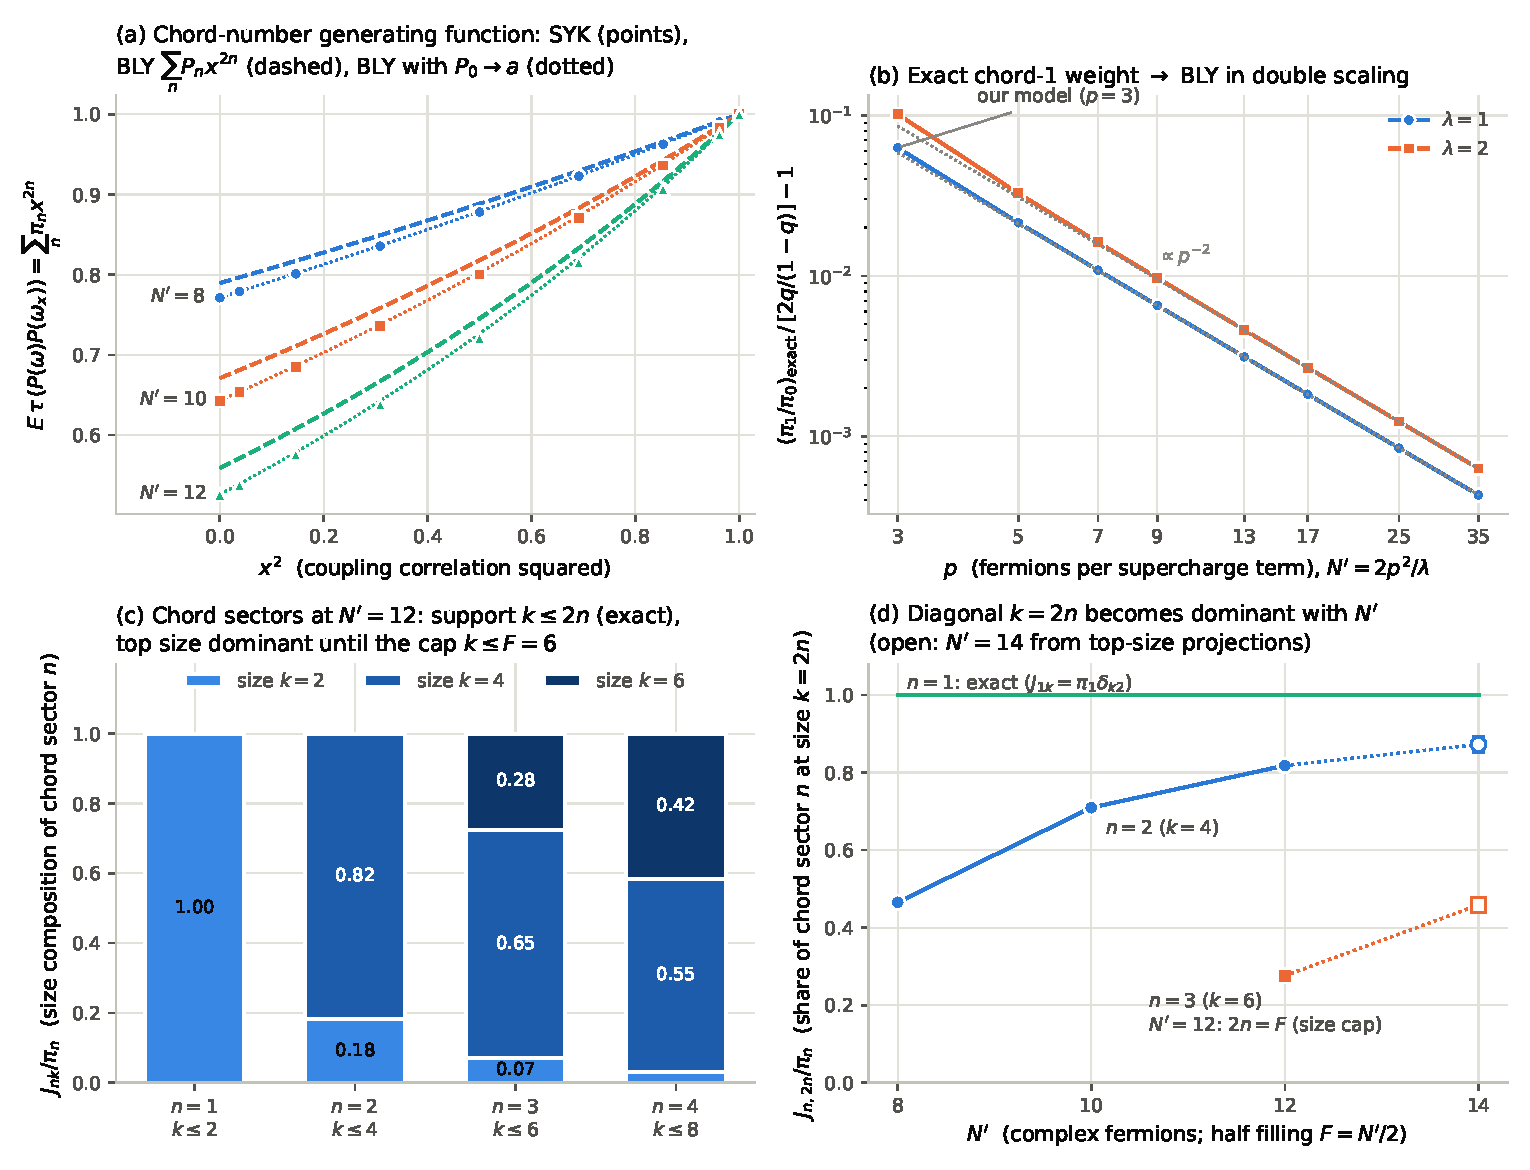
\includegraphics[width=\textwidth]{progress_2026-10-05_figs/fig_chord_size_dictionary.pdf}
\caption[The chord-number/size dictionary]{The chord-number/size dictionary.
\begin{itemize}\itemsep0pt
\item (a) \VER\ Generating function \eqref{eq:mehler} from angle-rotated OU pairs (points; errors smaller than markers).
  Dashed: BLY's $\sum_nP_nx^{2n}$ at $\lambda=18/\Np$. Dotted: the same with $P_0\to a$.
\item (b) \VER\ The exact chord-1 weight \eqref{eq:pi1} relative to BLY at fixed $\lambda$, approaching it as $p^{-2}$.
\item (c) \NUM\ Size composition $J_{nk}/\pi_n$ at $\Np=12$. The support $k\le2n$ is exact; $n=4$ is shown for
  completeness only (cutoff-sensitive).
\item (d) \NUM\ The share of the top size $k=2n$. Open symbols at $\Np=14$: top-size projections \eqref{eq:topsize}.
\end{itemize}}
\label{fig:dictionary}
\end{figure}

\FloatBarrier
%=====================================================================
\section{The fourth moment as a four-arc function}\label{sec:fourarc}
%=====================================================================
\subsection{One generating function for three coupling families \DER}
Let $K=\mathrm{diag}(K_J)$ be a real diagonal correlation on coupling space, $|K_J|\le1$, and let
$\tilde C=KC+\sqrt{1-K^2}\,C'$ with $C'$ an independent copy. Define
\begin{equation}
T_{2m}(K)=E\,\tau\big((P(C)P(\tilde C))^m\big).
\end{equation}
Three choices of $K$ concern us (Fig.~\ref{fig:rules}c):
\begin{itemize}\itemsep1pt
\item \textbf{OU family}, $K_J\equiv x$: all couplings partially resampled.
\item \textbf{Decoder}, $K_J=\sigma_J\equiv(-1)^{[i\in J]}$: deterministic. This is exact because $UQ(C)U=Q(\sigma C)$, hence
  $UP(C)U=P(\sigma C)$ (tested to $10^{-10}$). The parity family $U_A$ has $\sigma_J=(-1)^{|A\cap J|}$.
\item \textbf{Site-local family}, $K_J=z$ for $J\ni i$ and $1$ otherwise. Only the couplings touching site $i$ are
  resampled. Then $z=0$ is a fresh draw of those couplings, and $z=-1$ is the decoder.
\end{itemize}
Writing $F(C)=P(C)\otimes P(C)$ and $\mathcal B(A\otimes B,C\otimes D)=\tau(ACBD)$, the multivariate Mehler formula
(valid also at $|K_J|=1$, by parity of Hermite polynomials) gives
\begin{equation}
\boxed{\;T_4(K)=\sum_\alpha K^\alpha\,t_\alpha,\qquad t_\alpha=\mathcal B(F_\alpha,F_\alpha)\;}
\label{eq:genfun}
\end{equation}
Here $\alpha$ runs over multi-indices of Wick contractions between arcs of different flavour. \textbf{The three
families evaluate the same coefficients $t_\alpha$ at different points $K$.} Unlike $\pi_n$, the $t_\alpha$ need not be
positive: $T_4=\tau(Z^2)$ with $Z=P(C)P(\tilde C)$, whereas the time-ordered $\tau(Z^\dagger Z)$ is a norm.

\subsection{The four-arc rule, and why it is not random matter \DER}
Contractions between the two $C$-arcs are internal to $F_\alpha$ and carry 1. So on a circle with arcs
$P,P',P,P'$:
\begin{itemize}\itemsep1pt
\item chords between \emph{adjacent} arcs carry $K_J$;
\item chords between \emph{opposite} arcs carry 1.
\end{itemize}
This is the 29 September $\mathbb Z_2$ rule, now with an exact finite-$N$ realization by Gaussian couplings
(Fig.~\ref{fig:rules}a). For a fixed $\mathbb Z_2$ probe all three pairings of the four $U$'s give the same sign,
$(-1)^{\#U\text{ between the chord ends}}$, so there is no sum over $U$-pairings.

For BINT's random matter $M$ (independent couplings, crossing weight $\tilde q=e^{-2pp_M/N}$ per $H$-chord), an $H$-chord
between opposite arcs crosses both $M$-chords and carries $\tilde q^{\,2}$ (Fig.~\ref{fig:rules}b; BINT eqs.~2.9--2.11,
4.10--4.13~\cite{BINT}). The crossed four-point function and its $U_q(\mathfrak{su}(1,1))$ R-matrix (their 5.6) therefore
do \emph{not} give $T_4$ by substituting $\tilde q=x$. What is needed is the crossing kernel of the $\mathbb Z_2$ rule,
which is not in the literature we have.

\begin{figure}[!tbp]
\centering
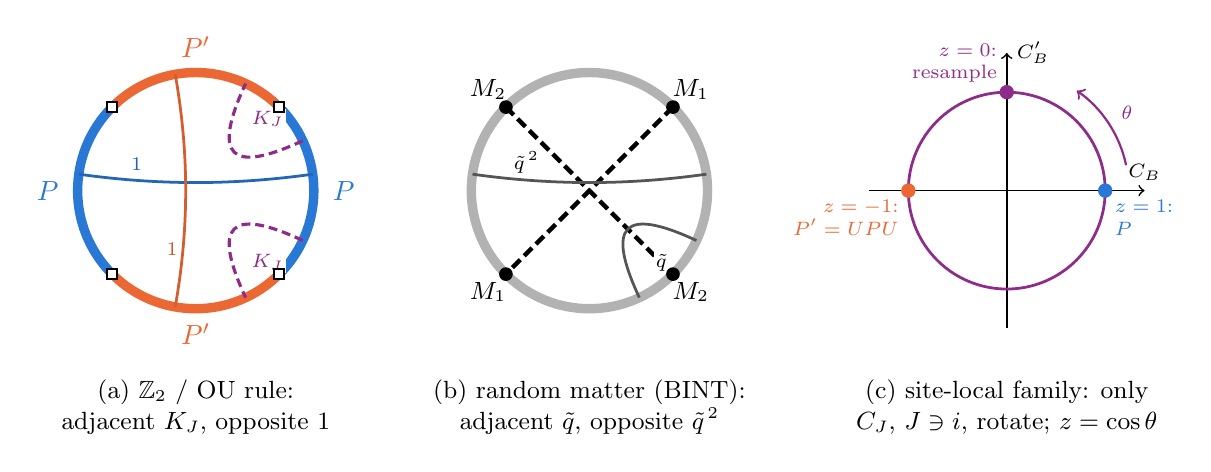
\begin{tikzpicture}
\def\R{1.5}
% (a) Z2 / OU rule
\begin{scope}
  \draw[Parc] (-45:\R) arc[start angle=-45, end angle=45, radius=\R];
  \draw[Pparc] (45:\R) arc[start angle=45, end angle=135, radius=\R];
  \draw[Parc] (135:\R) arc[start angle=135, end angle=225, radius=\R];
  \draw[Pparc] (225:\R) arc[start angle=225, end angle=315, radius=\R];
  \chord[chP]{8}{172}{\R}
  \chord[chX]{25}{65}{\R}
  \chord[chX]{-25}{-65}{\R}
  \chord[chPp]{100}{260}{\R}
  \node[cX, fill=white, inner sep=0.8pt] at (45:0.86*\R) {\scriptsize $K_J$};
  \node[cX, fill=white, inner sep=0.8pt] at (-45:0.86*\R) {\scriptsize $K_J$};
  \node[cP!80!black, fill=white, inner sep=0.8pt] at (-0.75,0.33) {\scriptsize $1$};
  \node[cPp!85!black, fill=white, inner sep=0.8pt] at (-0.30,-0.75) {\scriptsize $1$};
  \Umk{45}{\R}\Umk{135}{\R}\Umk{225}{\R}\Umk{315}{\R}
  \node[cP] at (0:\R+0.38) {$P$}; \node[cP] at (180:\R+0.38) {$P$};
  \node[cPp] at (90:\R+0.32) {$P'$}; \node[cPp] at (270:\R+0.32) {$P'$};
  \node[align=center, font=\small] at (0,-2.75) {(a) $\mathbb Z_2$ / OU rule:\\ adjacent $K_J$, opposite $1$};
\end{scope}
% (b) BINT random matter
\begin{scope}[xshift=5.0cm]
  \draw[Harc] (-45:\R) arc[start angle=-45, end angle=315, radius=\R];
  \chord[chM]{45}{225}{\R}
  \chord[chM]{135}{315}{\R}
  \chord[chH]{8}{172}{\R}
  \chord[chH]{-25}{-65}{\R}
  \node[fill=white, inner sep=0.8pt] at (-0.80,0.36) {\scriptsize $\tilde q^{\,2}$};
  \node[fill=white, inner sep=0.8pt] at (-45:0.86*\R) {\scriptsize $\tilde q$};
  \Mmk{45}{\R}\Mmk{135}{\R}\Mmk{225}{\R}\Mmk{315}{\R}
  \node at (45:\R+0.32) {\small $M_1$}; \node at (225:\R+0.32) {\small $M_1$};
  \node at (135:\R+0.32) {\small $M_2$}; \node at (315:\R+0.32) {\small $M_2$};
  \node[align=center, font=\small] at (0,-2.75) {(b) random matter (BINT):\\ adjacent $\tilde q$, opposite $\tilde q^{\,2}$};
\end{scope}
% (c) site-local coupling family
\begin{scope}[xshift=10.3cm]
  \draw[->, line width=0.6pt] (-1.75,0) -- (1.75,0) node[above, font=\scriptsize] {$C_B$};
  \draw[->, line width=0.6pt] (0,-1.75) -- (0,1.75) node[right, font=\scriptsize] {$C'_B$};
  \draw[line width=1.0pt, cX] (0,0) circle (1.25);
  \fill[cP] (1.25,0) circle (2.6pt) node[below right, font=\scriptsize, cP, align=left] {$z=1$:\\ $P$};
  \fill[cX] (0,1.25) circle (2.6pt) node[above left, font=\scriptsize, cX, align=right] {$z=0$:\\ resample};
  \fill[cPp] (-1.25,0) circle (2.6pt) node[below left, font=\scriptsize, cPp, align=right] {$z=-1$:\\ $P'=UPU$};
  \draw[->, line width=0.8pt, cX] (12:1.55) arc[start angle=12, end angle=55, radius=1.55];
  \node[font=\scriptsize, cX] at (33:1.82) {$\theta$};
  \node[align=center, font=\small] at (0,-2.75) {(c) site-local family: only\\ $C_J$, $J\ni i$, rotate; $z=\cos\theta$};
\end{scope}
\end{tikzpicture}
\caption[Four-arc chord rules and coupling families]{\DER\ Four-arc chord rules and coupling families.
\begin{itemize}\itemsep0pt
\item (a) In $T_4=\tau(PP'PP')$, chords between adjacent arcs carry the coupling correlation $K_J$: $x$ for OU pairs,
  $(-1)^{[i\in J]}$ for the decoder. Chords between opposite arcs carry 1.
\item (b) For BINT's random matter, an $H$-chord between opposite arcs crosses both matter chords and carries
  $\tilde q^{\,2}$. The two rules differ, so the random-matter R-matrix does not apply.
\item (c) The site-local family rotates only the couplings touching site $i$ in the plane $(C_B,C'_B)$. Its antipode is
  exactly the decoder. The OU family rotates all couplings in the plane $(C,C')$, with $x=\cos\theta$ and
  $P(-C)=P(C)$.
\end{itemize}}
\label{fig:rules}
\end{figure}

\subsection{When is the decoder an OU pair? \DER}
By $S_N$ invariance the site-averaged decoder weight of a multi-index $\alpha$ is
\begin{equation}
E_i[\sigma^\alpha]=1-\frac{2\,o(\alpha)}{N},\qquad\text{more generally}\quad E_{|A|=s}[\sigma^\alpha]=\frac{\mathcal K_s(o(\alpha))}{\binom Ns},
\end{equation}
where $o(\alpha)$ is the number of sites covered an odd number of times by the cross-chords' index sets (the support of
the monomial $\prod\psi$) and $\mathcal K_s$ is a Krawtchouk polynomial.
\begin{itemize}\itemsep1pt
\item For \emph{independent uniformly random} index sets, $E[\sigma^\alpha]=x_s^{|\alpha|}$ exactly, with
  $x_s=\mathcal K_s(p)/\binom Ns$. So \emph{the decoder equals OU at $x_s$, coefficient by coefficient, exactly when the
  cross-chord index sets are uncorrelated.}
\item \textbf{Double scaling with a heavy probe} ($s\propto\sqrt N$, $p^2/N$ fixed). Overlap correlations shift $o$ by
  $O(1)$ and change the weights by $O(s/N)\to0$, so decoder $\equiv$ OU$(x_s)$ for every $T_{2m}$ at leading order. A
  single-site probe trivializes there ($x_s\to1$).
\item \textbf{Finite $p$.} The correlations are large: the chord-1 weight is $\hat\chi_2(U)$, not $x_s^2$
  (\S\ref{sec:selection}). The meaningful comparison is therefore at the \emph{matched} $x_*$ defined by
  $T_2^\OU(x_*)=T_2^\dec$. At chaos order $\le1$ this predicts $x_*\approx\sqrt{\hat\chi_2(U)}$.
\end{itemize}

\subsection{Exact properties of the OU curve \DER}
\begin{itemize}\itemsep1pt
\item $T_2^\OU=\sum_n\pi_nx^{2n}$ and $T_4^\OU=\sum_n\theta_nx^{2n}$, even since $P(-C)=P(C)$. $T_4(1)=1$ and
  $T_4(0)=c_0$.
\item \textbf{Sum rule.} $\sum_nn\,\theta_n=2\sum_nn\,\pi_n$, since $\partial_xT_4=2\partial_xT_2$ at $x=1$ by $P^2=P$.
\item \textbf{Remainder.} With $Y_x=P_x-a$, the split $Q_4=S+R$ of 29 September applies along the curve. At $x=0$,
  $E_{C'}|Y'\rangle\rangle\langle\langle Y'|$ is $U(N)$-invariant and hence orthogonal to $\delta\mathcal P$, so
  $R^\OU(0)=0$ exactly. Also $R^\OU(1)=(1-a)^2-S$.
  \begin{itemize}\itemsep1pt
  \item \NUM\ $S^\OU(x)=E\sum_k\phi_k(\omega)w_k(\omega_x)$ depends on $x$ only through covariances of per-realization
    size data. These are $\le8\times10^{-7}$ at $\Np=8$--14, so $S$ is effectively $x$-independent.
  \end{itemize}
\item \textbf{$\sin^4$ identity.} $T_4-2T_2+1=\tau\big((PP_xP-P)^2\big)=E\sin^4\theta$ over principal angles. For the
  decoder this is $4\tau((PP_oP)^2)$ with $P_o=(P-UPU)/2$.
\item \textbf{Small angle} ($\epsilon=1-x$, real coordinates $\omega_I$ of unit variance). $PP_xP-P=-B^\dagger B+O(\delta\omega^3)$
  with $B=\sum_I\delta\omega_I(1-P)\partial_IP\,P$. Hence
  \begin{equation}
  1-T_2\simeq\frac{2\epsilon}{d}E\,\Tr g_{\rm tot},\qquad
  T_4-2T_2+1\simeq\frac{4\epsilon^2}{d}E\Big[\Tr g_{\rm tot}^2+2\sum_{IJ}\Tr g_{IJ}^2\Big].
  \label{eq:smallangle}
  \end{equation}
  Here $G_{IJ}=P\partial_IP(1-P)\partial_JP\,P$ is the operator-valued quantum geometric tensor (Chen et al.~\cite{CCMP},
  App.~A), $g_{IJ}=(G_{IJ}+G_{JI})/2$ and $g_{\rm tot}=\sum_Ig_{II}$.
  \begin{itemize}\itemsep1pt
  \item The Berry curvature $F_{IJ}=G_{IJ}-G_{JI}$ cancels between the $IJIJ$ and $IJJI$ Wick orderings.
  \item So isotropic noise measures the variance of the quantum metric, not the curvature moment $\Tr FF^\dagger$, which G.~Lin
    writes as TOC$-$OTOC~\cite{GLin} (his 6.15--6.19).
  \item The ratio $\kappa\equiv(T_4-2T_2+1)/(1-T_2)^2\to d\,E[\cdots]/(E\Tr g_{\rm tot})^2$ is the normalized
    heterogeneity of the BPS states' sensitivity.
  \end{itemize}
\item \textbf{Conjugation flow.} $P(\theta)=e^{i\theta n_i}Pe^{-i\theta n_i}$ interpolates $P\to P'$, a conjugation
  deformation in the sense of~\cite{CCMP}. Its quantum metric is $\hat\Lambda(1-\hat\Lambda)$ with
  $\hat\Lambda=Pn_iP=P-O$, and $T_2(\theta)=1-2(1-\cos\theta)\,\tau(\hat\Lambda-\hat\Lambda^2)$ exactly.
\end{itemize}

\subsection{Two-sided reading \DER\ (double-scaled Majorana) + \INTERP\ ($\mathcal N=2$)}
In the $q$-Gaussian GNS space left and right multiplications commute. Hence
\begin{equation}
T_4^\OU=\langle\Psi_{h_x,h}|\Psi_{h,h_x}\rangle,\qquad |\Psi_{h,h'}\rangle=L\big(P(h)\big)\,R\big(P(h')\big)\,\Omega ,
\end{equation}
\begin{itemize}\itemsep1pt
\item $|\Psi_{h,h'}\rangle$ is the zero-energy state of the two-sided chord Hilbert space~\cite{Lin22}. Its left
  boundary evolves with $H(\omega)$ and its right boundary with $H(\omega_x)$. Chords are coloured by their emitting
  boundary, and the inner product is the $q$-Fock product with $\langle h,h_x\rangle=x$.
\item So \textbf{$T_4^\OU$ is the overlap of a mismatched BPS wormhole with its mirror}, and
  $T_2^\OU=\langle\Omega|\Psi_{h,h_x}\rangle$.
\item By BKS (\S4), $(P(\omega),P(\omega_x))$ are values of the $q$-OU process at two times. $T_2$ is time-ordered, but
  $T_4$ has operator times $(s,t,s,t)$: it is an out-of-time-order correlator of the $q$-OU process, not fixed by its
  Markov kernel.
\item At finite $N$ this identity is just vectorization. Its content is that the double-scaled limit is a two-colour
  chord computation, not a matter-chord R-matrix.
\item The $\mathcal N=2$ version (BBNR's oriented chords) follows by the same multilinearity, but we have not seen it
  written down.
\end{itemize}

\FloatBarrier
%=====================================================================
\section{The free-liberation baseline}\label{sec:liberation}
%=====================================================================
The natural Hilbert-space-isotropic null model rotates $P$ against itself by a free unitary Brownian motion $Y_t$,
free from $P$: the free Jacobi process $J_t=PY_tPY_t^*P$ with $\tau(P)=a$, i.e.\ Demni--Hamdi--Hmidi parameters
$\lambda=1$, $\theta=a$~\cite{DHH}. Their moment equation (eq.~2) is stated for any initial data; here $m_n(0)=1$. With
$u=e^{-t}$ and $b=1-a$ it gives \DER
\begin{gather}
T_2=a+b\,u\quad\Rightarrow\quad\eta\equiv\frac{T_2-a}{1-a}=e^{-t}\ \text{exactly},\nonumber\\
T_4=a^2(2-a)+4ab^2u+(E-2ab^2t)\,u^2,\qquad E=1-a^2(2-a)-4ab^2 .
\end{gather}
Relative to the free two-model value $c_0^{\rm free}=a^2(2-a)$ (i.e.\ $S_{\rm free}=a^2(1-a)$):
\begin{equation}
\boxed{\;R_\lib(\eta)=2a(1-a)(1-2a)\,\eta+\big[E+2a(1-a)^2\ln\eta\big]\eta^2\;}
\end{equation}
\begin{itemize}\itemsep1pt
\item \textbf{Checks.}
  \begin{itemize}\itemsep1pt
  \item It agrees with the numerically integrated ODE to $10^{-11}$, and $t\to\infty$ gives the Wachter value.
  \item $R_\lib(1)=1-2a+a^3=(1-a)^2-S_{\rm free}$.
  \item A finite-$D$ simulation ($D=800$--2000, unitary Brownian motion from GUE exponentials) reproduces the ODE moments
    to $\lesssim2\times10^{-3}$.
  \end{itemize}
\item \textbf{Sign structure.} The linear term changes sign at $a=\tfrac12$. $R(1)$ changes sign at the golden-ratio root
  $a=(\sqrt5-1)/2=0.618$ of $a^3-2a+1$. This is the threshold observed empirically on 29 September, where $\Np=8,10$
  ($a>0.618$) had $R<0$.
\item \textbf{Small angle.} $\kappa\to1/(1-a)$: free-Poisson statistics of $B^\dagger B$ for $B=(1-P)\,dW\,P$.
\item \textbf{Non-analyticity.} The $\eta^2\ln\eta$ term is non-analytic. The OU curve is a power series in $x^2$, so OU
  can approximate liberation but never equal it.
\end{itemize}

%=====================================================================
\section{Numerics: decoder vs OU vs free liberation}\label{sec:numerics}
%=====================================================================
\paragraph{Design.}
\begin{itemize}\itemsep1pt
\item Per sample, $K=16$ BPS projectors are built on a circle in coupling space (angle trick). For the OU family,
  $\omega_j=\cos\theta_j\,\omega+\sin\theta_j\,\omega'$ with $\theta_j=j\pi/K$, giving 9 values of $x$ including $x=0$
  exactly. For the site family, only $C_B$ rotates, with $\theta_j=2\pi j/K$, giving $z\in[-1,1]$; $z=-1$ \emph{is} the
  decoder.
\item cos$^2$ of the principal angles come from orthonormal BPS bases; moments $T_2$--$T_{16}$ and spectra are recorded.
\item On the same realizations the decoder (all $\Np$ single sites) and parity probes ($|A|=2..\Np/2$) are evaluated, so
  decoder and OU are \emph{realization-matched}.
\item Samples: 200, 150, 100, 60, 40, 16, 14 at $\Np=8$--14 (OU), and 150, 80, 30 at $\Np=8,10,12$ (site family).
  Errors are bootstrap over samples.
\item \textbf{Cross-checks.}
  \begin{itemize}\itemsep1pt
  \item The fitted $\pi_1$ reproduces \eqref{eq:pi1} (Table~\ref{tab:pi1}).
  \item The measured endpoints $c_0=T_4^\OU(0)$, namely 0.56428(50), 0.41581(71), 0.29420(126), 0.29744(52) at
    $\Np=10,12,13,14$, reproduce the 29 September parameter-free two-model predictions 0.56399, 0.41606, 0.29481,
    0.29661.
  \item $R_\dec$ agrees with the independent 29 September run: $+0.0121$ vs $+0.0119$ at $\Np=12$, $+0.0515$ vs $+0.0500$
    at 13, and $+0.0508$ vs $+0.0531$ at 14.
  \end{itemize}
\end{itemize}

\subsection{Isotropic deformations are close to free liberation \NUM}
\begin{table}[!htbp]
\centering\small
\begin{tabular}{@{}cccccc@{}}
\toprule
$\Np$ & $a$ & $q=e^{-18/\Np}$ & $\max_x(T_4^\OU-T_4^\lib)$ [at $x$] & same for $T_8$ & $c_0-c_0^{\rm free}$\\
\midrule
8 & 0.7714 & 0.105 & $-0.0025$ [0.383] & $-0.0028$ & $-0.0010$\\
9 & 0.6429 & 0.135 & $+0.0043$ [0.831] & $+0.0099$ & $+0.0025$\\
10 & 0.6429 & 0.165 & $+0.0031$ [0] & $+0.0057$ & $+0.0034$\\
11 & 0.5260 & 0.195 & $+0.0081$ [0.831] & $+0.0182$ & $+0.0079$\\
12 & 0.5260 & 0.223 & $+0.0083$ [0] & $+0.0165$ & $+0.0080$\\
13 & 0.4248 & 0.250 & $+0.0120$ [0.831] & $+0.0258$ & $+0.0099$\\
14 & 0.4248 & 0.276 & $+0.0121$ [0] & $+0.0222$ & $+0.0132$\\
\bottomrule
\end{tabular}
\caption{\NUM\ Largest deviation of the OU curve from free liberation at equal $T_2$, over the 8 lags. It tracks the
two-model non-freeness $c_0-c_0^{\rm free}$, and both grow with $q$, as Liu--Shen's inter-model crossing weight
$q_{12}=q$ suggests~\cite{LiuShen}. The bulk of the spectrum coincides with liberation (Fig.~\ref{fig:fourarc}d). OU has
a soft tail below the free lower edge.}
\label{tab:oulib}
\end{table}
At infinitesimal angle the heterogeneity ratio $\kappa$ of OU is 4.51, 3.02, 2.36 at $\Np=8,10,12$. The free values
$1/(1-a)$ are 4.38, 2.80, 2.11, so OU is $+3$, $+8$, $+12\,\%$ above free.

\subsection{The decoder exceeds the isotropic curve \NUM}
\begin{table}[!htbp]
\centering\footnotesize
\setlength{\tabcolsep}{2.6pt}
\begin{tabular}{@{}cccccccccc@{}}
\toprule
$\Np$ & $T_2^\dec$ & $x_*$ & $T_4^\dec$ & $T_4^\OU(x_*)$ & $T_4^\lib$ & $T_4^{\rm free}$ & liberation & isotropic & localization\\
\midrule
8 & 0.8174(2) & 0.476 & 0.7778(2) & 0.7603(2) & 0.7627 & 0.7311 & 0.0316 (68\,\%) & $-0.0024$ ($-5$\,\%) & 0.0175(1) (37\,\%)\\
9 & 0.7319(3) & 0.557 & 0.6666(3) & 0.6373(3) & 0.6354 & 0.5609 & 0.0745 (70\,\%) & $+0.0019$ (2\,\%) & 0.0293(1) (28\,\%)\\
10 & 0.7456(3) & 0.582 & 0.6790(3) & 0.6469(3) & 0.6475 & 0.5609 & 0.0867 (73\,\%) & $-0.0006$ ($-1$\,\%) & 0.0321(1) (27\,\%)\\
11 & 0.6690(3) & 0.630 & 0.5799(4) & 0.5419(3) & 0.5356 & 0.4078 & 0.1278 (74\,\%) & $+0.0064$ (4\,\%) & 0.0380(2) (22\,\%)\\
12 & 0.6861(3) & 0.650 & 0.5964(3) & 0.5548(3) & 0.5519 & 0.4078 & 0.1441 (76\,\%) & $+0.0029$ (2\,\%) & 0.0417(2) (22\,\%)\\
13 & 0.6184(5) & 0.684 & 0.5101(5) & 0.4669(5) & 0.4562 & 0.2843 & 0.1719 (76\,\%) & $+0.0107$ (5\,\%) & 0.0432(2) (19\,\%)\\
14 & 0.6368(4) & 0.696 & 0.5283(4) & 0.4816(4) & 0.4742 & 0.2843 & 0.1900 (78\,\%) & $+0.0074$ (3\,\%) & 0.0467(2) (19\,\%)\\
\bottomrule
\end{tabular}
\caption{\NUM\ The decoder ($s=1$) at equal $T_2$. $T_4^{\rm free}=2a^2-a^3$ (Wachter), and $T_4^\lib$ is free liberation
at $T_2^\dec$. The excess $T_4^\dec-T_4^{\rm free}$ splits into liberation $=T_4^\lib-T_4^{\rm free}$, isotropic
$=T_4^\OU(x_*)-T_4^\lib$ and localization $=T_4^\dec-T_4^\OU(x_*)$. Parentheses: bootstrap SE in units of
$10^{-4}$.}
\label{tab:split}
\end{table}

\begin{itemize}\itemsep1pt
\item The localization term grows but saturates in absolute size (0.017, 0.032, 0.042, 0.047 at even $\Np=8$--14), while
  its share falls from 37 to 19\,\%.
\item $T_6$ and $T_8$ show the same pattern with larger excesses. At $\Np=14$: $T_6$ 0.469 vs 0.394, $T_8$ 0.430 vs 0.337.
  The decoder's principal angles are more heterogeneous.
\item \textbf{Matched OU parameter.} $x_*=$ 0.476, 0.557, 0.582, 0.630, 0.650, 0.684, 0.696 against
  $\sqrt{\hat\chi_2(U)}=$ 0.471, 0.537, 0.588, 0.628, 0.660, 0.688, 0.711 ($\Np=8$--14). The naive $x_s=1-2p/\Np$ is
  0.25--0.57.
\item \textbf{Parity family.} For $|A|=s>1$ the excess is smaller in absolute terms but larger \emph{relative} to the OU
  distance from independence: 0.30, 0.43, 0.65 for $s=1,2,3$ at $\Np=12$. Heavier parity probes are thus not ``more
  isotropic'' at these sizes. This does not contradict the double-scaling statement of \S\ref{sec:fourarc}, which needs
  $s/N\to0$ with $p\propto\sqrt N$.
\end{itemize}

\subsection{The excess is localization, not the $\mathbb Z_2$ sign \NUM}
\begin{table}[!htbp]
\centering\footnotesize
\begin{tabular}{@{}ccccc|cccc@{}}
\toprule
& \multicolumn{4}{c|}{excess of $T_4$ over the OU curve at equal $T_2$} & \multicolumn{4}{c}{small-angle $\kappa$}\\
$\Np$ & $z=0.707$ & $z=0$ (resample) & $z=-1$ (decoder) & $z=0$ share & $1/(1-a)$ & OU & site & site/free\\
\midrule
8 & 0.0021 & 0.0121 & 0.0174 & 0.69 & 4.38 & 4.51 & 5.36 & $+22\,\%$\\
10 & 0.0039 & 0.0213 & 0.0324 & 0.66 & 2.80 & 3.02 & 3.86 & $+38\,\%$\\
12 & 0.0057 & 0.0279 & 0.0414 & 0.67 & 2.11 & 2.36 & 3.15 & $+49\,\%$\\
\bottomrule
\end{tabular}
\caption{\NUM\ The site-local family $T(1,z)$. Its $z=-1$ endpoint reproduces the decoder's excess (Table~\ref{tab:split})
within errors. Gaussian resampling of only the site's couplings ($z=0$, no $\mathbb Z_2$ sign) already gives two thirds
of it. The excess grows smoothly from the identity, $\propto(1-T_2)^2$ near $z=1$, as \eqref{eq:smallangle} requires.
$\kappa$ is evaluated at the point nearest the identity: $x=0.981$ (OU) and $z=0.924$ (site).}
\label{tab:site}
\end{table}

\begin{figure}[!tbp]
\centering
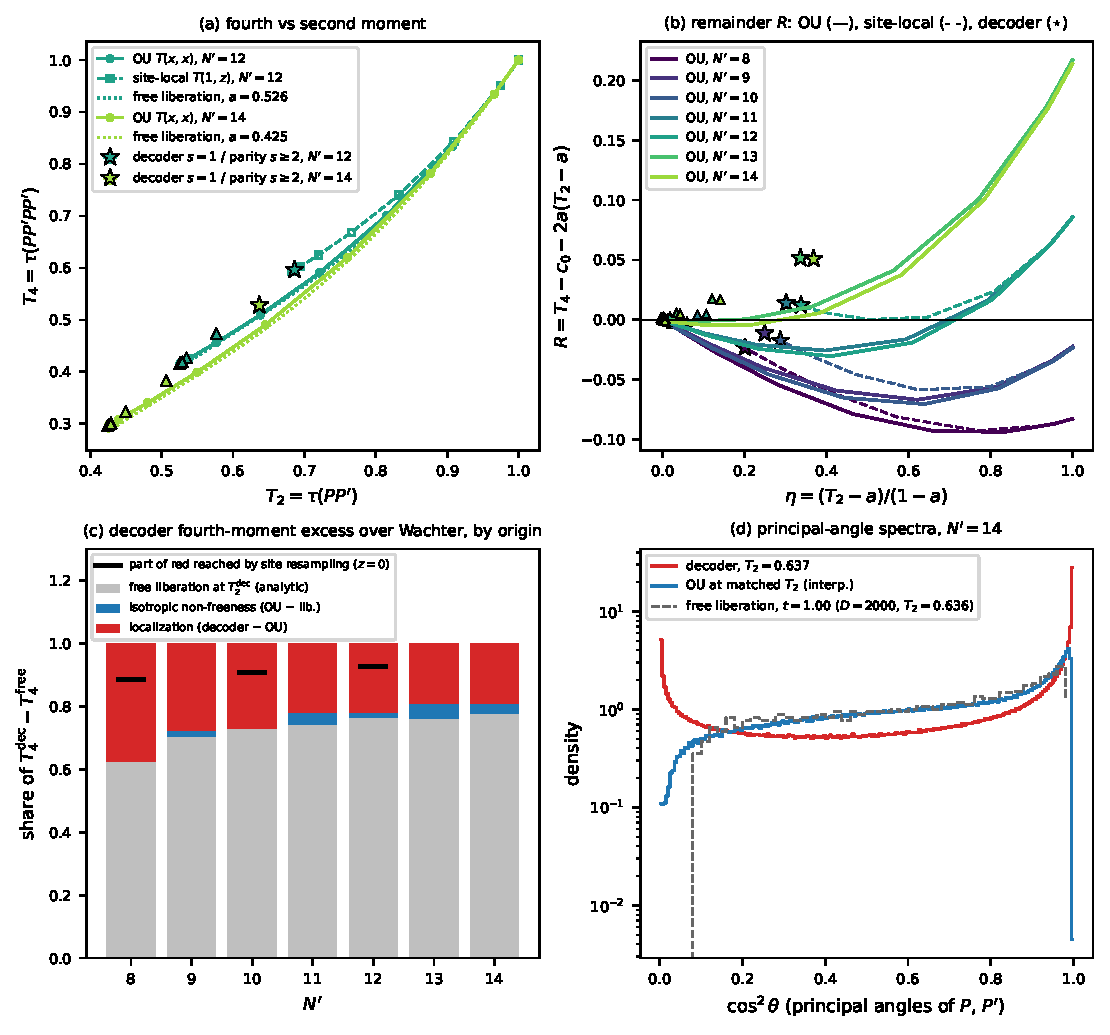
\includegraphics[width=\textwidth]{progress_2026-10-05_figs/fig_ou_fourarc.pdf}
\caption[Decoder vs isotropic and site-local deformations]{\NUM\ Decoder vs isotropic and site-local deformations.
\begin{itemize}\itemsep0pt
\item (a) $T_4$ against $T_2$: OU family (solid), site-local family (dashed), free liberation (dotted), decoder ($\star$)
  and parity probes ($\blacktriangle$), at $\Np=12,14$.
\item (b) $R=T_4-c_0-2a(T_2-a)$ against $\eta=(T_2-a)/(1-a)$ for all $\Np$. The sign of the OU curves flips between
  $a>\tfrac12$ and $a<\tfrac12$, as $R_\lib$ predicts.
\item (c) The three-way split of Table~\ref{tab:split}. Black ticks: how much of the localization (red) the site
  resampling $z=0$ reaches.
\item (d) Principal-angle spectra at $\Np=14$: the decoder, OU at matched $T_2$ (histograms interpolated between
  neighbouring lags), and finite-$D$ free liberation ($D=2000$) at $t=-\ln\eta$. OU and liberation coincide in the bulk;
  the decoder is dominated by wall pile-ups at $\cos^2\theta\in\{0,1\}$.
\end{itemize}}
\label{fig:fourarc}
\end{figure}

\FloatBarrier
%=====================================================================
\section{What $R$ is, and what a gravity computation should target}\label{sec:gravity}
%=====================================================================
\subsection{Decomposition of $R$}
At equal $T_2$,
\begin{equation}
R_\dec=\underbrace{R_\lib(\eta)}_{\text{analytic}}+\underbrace{\delta_{\rm iso}}_{R^\OU(x_*)-R_\lib}+\underbrace{\delta_{\rm loc}}_{T_4^\dec-T_4^\OU(x_*)} .
\end{equation}
At $\Np=12$ ($\eta=0.338$) the three terms are $-0.024$, $-0.005$ and $+0.042$, summing to $R_\dec=+0.012$. The 29 September $R$ was opaque
because it is a small difference of a large negative free-probability piece and a large positive local piece. The two
closures tried then (size-diagonal characters; a coherent mixture) were closures of this sum; neither separates the
pieces.

\subsection{Mechanism of the localization term \INTERP, grounded in \S\ref{sec:fourarc}}
\begin{itemize}\itemsep1pt
\item The decoder weight of a chaos component is $1-2o(\alpha)/N$; isotropic OU weighs it $x^{|\alpha|}$. The two agree
  when cross-chord index sets are independent.
\item In $\mathcal N=2$ SYK, $\{\psi_J,\psi_K^\dagger\}=0$ for disjoint $J,K$, so the chaos content of $P$ is built from
  overlapping index-set pairs ($P_{[1]}\propto H^{(2)}$). Chords through site $i$ therefore cluster. The number of
  probe-sensitive chords is then overdispersed relative to an isotropic deformation. At fixed mean (equal $T_2$) this
  raises $E\sin^4\theta$.
\item Spectrally this is the wall pile-up: BPS states in which site $i$ is effectively frozen or maximally uncertain. It
  is the UV imprint of $n_i$ on the LMRS operator $Pn_iP$, cf.\ Chen et al.'s Fig.~5a~\cite{CCMP}. Infinitesimally it is the excess heterogeneity
  $\kappa$ of the site-restricted quantum metric.
\end{itemize}

\subsection{Gravitational reading \INTERP}
\begin{itemize}\itemsep1pt
\item \textbf{Universal part.} The isotropic four-arc function is the overlap of mismatched two-sided BPS wormholes. At
  $\Np\le14$ ($q\approx0.1$--0.3) it is close to free liberation.
  \begin{itemize}\itemsep1pt
  \item \CONJ\ The double-scaled isotropic function is a $q$-deformed liberation that reduces to the free one as $q\to0$.
    Its departure from free is set by the two-model crossing weight $q_{12}=q$.
  \item A dynamical reading: \emph{generic coupling changes rotate the BPS space like a free unitary Brownian motion}.
    This is a dynamical form of the Haar-orientation (BPS-chaos) hypothesis of Belin--Fu--La~Rocca~\cite{BFL}.
  \end{itemize}
\item \textbf{Local part.} It vanishes in strict double scaling (a single-site probe trivializes; for heavy probes
  decoder $\equiv$ OU). It is a finite-$p$, site-resolved effect that neither structureless matter chords (BINT/BLY) nor
  super-JT capture.
  \begin{itemize}\itemsep1pt
  \item The exact zero-energy $\mathcal N=2$ OTOC now available (G.~Lin, eqs.~5.26--5.38~\cite{GLin}) is the
    triple-scaled limit of the isotropic, universal part at best.
  \item LMRS's large-$\Delta$ suppression of crossed diagrams (their eq.~159~\cite{LMRS}) is irrelevant for our light
    probe.
  \end{itemize}
\item \textbf{Consequence for 7.3.2.} The chord computation should target $T_4^\OU(x)$, which is universal and
  liberation-like, with the localization treated as a separate finite-$p$ correction. A single ``$\mathbb Z_2$ flag per
  chord'' calculation is not expected to reproduce the decoder's $R$ at $p=3$.
\end{itemize}

\begin{table}[!htbp]
\centering\small
\begin{tabular}{@{}>{\raggedright\arraybackslash}p{0.36\textwidth}>{\raggedright\arraybackslash}p{0.33\textwidth}>{\raggedright\arraybackslash}p{0.24\textwidth}@{}}
\toprule
exact finite-$N$ object & chord / gravity counterpart & status\\
\midrule
chaos degree $n$ of $P(\omega)$ & BLY chord number ($n$ XO pairs) & exact; $\pi_0=a$; $\pi_1\to$ BLY\\
$\mathrm{supp}\,J\subset\{k\le(p-1)n\}$ & BLY $\mathrm{size}_O=p\,n_O$ & exact; shift $p\to p-1$ (friend mode)\\
$\kappa_n=a\,p_n(0)^2$ & $P_n=a_\lambda p_n^{\rm DS}(0)^2$ & exact both; $\kappa\approx\pi$\\
$\hat\chi_2(U)$ on chord 1 & $q^{2\Delta}$ per chord pair & exact vs double-scaled\\
OU correlation $x$ & matter weight $\tilde q$ ($x^{\hat N}$) & exact (BKS, Pluma--Speicher)\\
$T_4^\OU(x)$ & overlap of mismatched BPS wormholes; $q$-OU OTOC & structural (double scaling)\\
$T_4^\OU$ vs $T_2^\OU$ & free liberation ($q\to0$?) & numerical, deviation $\le0.012$\\
decoder $-$ OU at equal $T_2$ & site-resolved chord clustering & numerical; absent in DS\\
$R_\lib(\eta)$ & free Jacobi process & exact, closed form\\
\bottomrule
\end{tabular}
\caption{Dictionary update. It replaces the rows ``size spectrum $\leftrightarrow P_n$: empirical'' and ``decoder $R$:
open'' of the 29 September Table~6.}
\label{tab:dictionary}
\end{table}

\subsection{Next computations}
\begin{enumerate}\itemsep1pt
\item \textbf{Analytic model of the localization term.} Start from \eqref{eq:smallangle} restricted to the couplings
  through site $i$, i.e.\ the variance of the site-restricted quantum-metric operator. Then extend to finite angle along the
  site family.
\item \textbf{Two-colour chord computation of $T_4^\OU(x)$} in BBNR/BLY double scaling (the mismatched-wormhole overlap).
  Test ``$q$-deformed liberation'': $q\to0$ should give the free Jacobi curve.
\item \textbf{$\Np=15$--16} with the BLAS3 basis, for the large-$\Np$ trend of the localization share.
\item \textbf{Finite-$N$ HH recursion for $\pi_n$, $n\ge2$} (open since 2 October): the chaos projections of
  $QP=PQ=0$.
\end{enumerate}

%=====================================================================
\section{Open questions and caveats}\label{sec:open}
%=====================================================================
\begin{enumerate}\itemsep2pt
\item \textbf{OU $\approx$ liberation is empirical.} It holds at $\Np\le14$, i.e.\ at small $q$, with deviations growing with
  $q$. The OU curve cannot equal liberation exactly (non-analytic $\eta^2\ln\eta$). ``$q$-deformed liberation'' is a
  conjecture.
\item \textbf{No analytic model of the localization term yet.} Its mechanism (chord clustering) is an interpretation
  supported by the exact weight formula, not a calculation. Its large-$\Np$ fate is open. The share falls, the absolute
  size appears to saturate, and in strict double scaling it should vanish.
\item \textbf{Two-sided reading.} It is derived for the double-scaled Majorana $q$-Gaussian algebra. The $\mathcal N=2$,
  BPS-projector version is by analogy.
\item \textbf{Chaos coefficients of $T_4$.} The $\theta_n$ are not reliably determined by 9 lags (alternating, large).
  Only the curves are used.
\item \textbf{$\Np=14$ statistics.} 14 OU samples, using 4 of the 16 pairs per lag. The site family stops at $\Np=12$.
\item \textbf{Liberation is a $D\to\infty$ model.} Finite-$D$ (Weingarten) corrections are $O(D^{-2})$ and negligible
  here, but the free Jacobi density for general $a$ is only simulated, not computed in closed form.
\item \textbf{Superseded.}
  \begin{itemize}\itemsep1pt
  \item ``$w_{2n}\leftrightarrow P_n$ is an empirical match'': replaced by \S\ref{sec:selection}.
  \item ``Per-chord weights factorize in double scaling'': replaced by the character $\hat\chi_2$.
  \item ``Correlated couplings need a correlated mixed $q$-Gaussian beyond Bożejko--Speicher'': wrong, see \S\ref{sec:chaos}.
  \item ``Two-copy irrep content of $R$'' (29 September item 7.3.3): deprioritized, since $R$ is now understood as a sum
    of two pieces with different origins.
  \end{itemize}
\end{enumerate}

\appendix
\section{Derivation details}
\subsection{Mehler formula for a diagonal correlation}
For a single complex Gaussian coordinate with $\tilde c=kc+\sqrt{1-k^2}c'$, the Hermite polynomials $H_{m,n}(c,\bar c)$
satisfy $E[H_{m,n}(\tilde c)\,|\,c]=k^{m+n}H_{m,n}(c)$. For $|k|=1$ this is the parity
$H_{m,n}(-c)=(-1)^{m+n}H_{m,n}(c)$. Products over coordinates give $E[F(\tilde C)\,|\,C]=\sum_\alpha K^\alpha F_\alpha(C)$.
Pairing with $F(C)$ through the bilinear form $\mathcal B$ and using orthogonality of distinct chaoses gives
\eqref{eq:genfun}.

\subsection{Small-angle expansion}
Differentiate $P^2=P$:
\begin{itemize}\itemsep1pt
\item to first order, $P\partial_IP\,P=0$;
\item to second order, $P\partial_I\partial_JP\,P=-P(\partial_IP\partial_JP+\partial_JP\partial_IP)P$.
\end{itemize}
Hence $P(P_x-P)P=-B^\dagger B+O(\delta\omega^3)$ with $B=(1-P)\,(\sum_I\delta\omega_I\partial_IP)\,P$. The mean shift of
$\delta\omega$ is $O(\epsilon)$ and odd fluctuation moments vanish, so corrections are $O(\epsilon^3)$. With
$E\,\delta\omega_I\delta\omega_J=2\epsilon\,\delta_{IJ}$, Wick's theorem on $\Tr(B^\dagger B)^2$ gives the three orderings
$IIKK$, $IJIJ$, $IJJI$. Writing $G_{IJ}=g_{IJ}+F_{IJ}/2$, the last two sum to $2\sum\Tr g_{IJ}^2$: the $\Tr F^2$ terms
cancel and the cross terms vanish by symmetry.

\subsection{Liberation closed form}
With $\lambda=1$ and $\theta=a$, DHH eq.~(2) reads
\begin{itemize}\itemsep1pt
\item $n=1$: $\dot m_1=-m_1+a$;
\item $n=2$: $\dot m_2=-2m_2+2am_1(2-m_1)$.
\end{itemize}
Insert $m_1=a+bu$. The $u^2$ term of the source is resonant with the homogeneous solution, which produces the
$t\,u^2=-u^2\ln u$ term. Fixing $m_2(0)=1$ gives $E$.

\section{Literature added in this cycle}\label{app:lit}
Notes are in \path{literature/notes/}, and \path{literature/synthesis.md} \S8 compares the tools. Each entry gives what
the paper establishes and how it is used here.
\begin{itemize}\itemsep1pt
\item \textbf{BBNR~\cite{BBNR}.}
  \begin{itemize}\itemsep1pt
  \item $\mathcal N=2$ double-scaled SYK: oriented chords, friend/enemy weights, the fixed-charge density, and the
    finite-$N$ ground-state count (our $d$).
  \item The double-chord rule $\tilde q^{\hat N}$.
  \item Four-point functions are listed there as open.
  \end{itemize}
\item \textbf{BINT~\cite{BINT}.}
  \begin{itemize}\itemsep1pt
  \item The matter-chord rule, the 2-point vertex (= $q$-Mehler kernel), and the crossed 4-point function with the
    $U_q(\mathfrak{su}(1,1))$ R-matrix.
  \item Its random-matter rule differs from ours (\S\ref{sec:fourarc}).
  \end{itemize}
\item \textbf{Pluma--Speicher~\cite{PS}.}
  \begin{itemize}\itemsep1pt
  \item Independent SYK copies $\to$ $q$-Gaussians; Brownian couplings $\to$ $q$-Brownian motion by multilinearity.
  \item Fluctuations at scale $\binom Np^{-1/2}$.
  \end{itemize}
\item \textbf{Bożejko--Kümmerer--Speicher~\cite{BKS}.} Second quantization $\Gamma_q(T)$; the $q$-OU process is Markov;
  classical versions reproduce only time-ordered correlators.
\item \textbf{G.~Lin~\cite{GLin}.} The exact zero-energy $\mathcal N=2$ super-JT OTOC for equal $\Delta$, and the
  Berry-curvature second moment as TOC$-$OTOC.
\end{itemize}

\section{Reproducibility}
All heavy runs were under \path{scripts/memwatch.py}; the peak was 1.43\,GB (at $\Np=14$).
\begin{center}\small
\begin{tabular}{@{}>{\raggedright\arraybackslash}p{0.28\textwidth}>{\raggedright\arraybackslash}p{0.67\textwidth}@{}}\toprule
Item & Code / data\\\midrule
Chord/size dictionary (\S\S\ref{sec:chaos}--\ref{sec:selection}, Fig.~\ref{fig:dictionary}) & \path{src/chord_chaos.py}, \path{src/plethysm.py}, \path{scripts/run_chord_chaos.py}, \path{analyze_chord_chaos.py}, \path{run_topsize_projection.py}, \path{run_chord1_sizes.py}, \path{plot_chord_size_dictionary.py}; data \path{results/data/chord_chaos_2026-10-01/}; tests \path{tests/test_chord_chaos.py}\\
OU / site / decoder (\S\ref{sec:numerics}, Fig.~\ref{fig:fourarc}) & \path{scripts/run_ou_fourarc.py}, \path{analyze_ou_fourarc.py}, \path{plot_ou_fourarc.py}; data \path{results/data/ou_fourarc_2026-10-05/} (incl.\ \path{analysis.json}, \path{analysis_output.txt}); tests \path{tests/test_ou_fourarc.py}\\
Notes & \path{research/notes/chord_size_dictionary_2026-10-02.md}, \path{research/notes/decoder_T4_fourarc_2026-10-05.md}; \path{docs/derivations.md} D4, D5\\
\bottomrule
\end{tabular}
\end{center}
\paragraph{Seeds and samples.} $p=3$ and $F=\lfloor\Np/2\rfloor$ throughout.
\begin{itemize}\itemsep1pt
\item \textbf{Dictionary campaign:} seeds $1000003(s_0+s)+17$.
  \begin{itemize}\itemsep1pt
  \item 4000/744/174 samples at $\Np=8/10/12$ ($K=16$);
  \item 5 samples at $\Np=14$ ($K=12$);
  \item top-size projections with 40 realizations (seed 41).
  \end{itemize}
\item \textbf{Four-arc campaign:} seeds $1000003(s_0+s)+29$; $s_0=0$ for OU and 1000 for the site family.
  \begin{itemize}\itemsep1pt
  \item Probe sets use seed$+7$.
  \item $\Np=14$ used the BLAS3 (Gram-eigh) basis and 4 pair starts per lag. That basis is identical to the Hodge/SVD
    basis to $3\times10^{-15}$.
  \end{itemize}
\item \textbf{Code states:} data generated at \texttt{ee619d3} (dictionary) and \texttt{1aa3dd3} plus working tree
  (four-arc), recorded in \path{meta_*.json}. This report is at \texttt{4395248} plus this file.
\end{itemize}

\begin{thebibliography}{99}\small
\bibitem{prog0929} \texttt{syk\_gravity} project, \emph{Progress report, 29 September 2026}, \path{research/pdfs/progress_2026-09-29.pdf}.
\bibitem{CV} J.~Chryssanthacopoulos and D.~Vegh, \emph{Fortuity and fragility in supersymmetric SYK}, arXiv:2608.12160 (2026).
\bibitem{BLY} J.~Boruch, H.~W.~Lin and C.~Yan, \emph{Exploring supersymmetric wormholes in $\mathcal N=2$ SYK with chords}, JHEP 12 (2023) 151, arXiv:2308.16283.
\bibitem{BBNR} M.~Berkooz, N.~Brukner, V.~Narovlansky and A.~Raz, \emph{The double scaled limit of super-symmetric SYK models}, JHEP 12 (2020) 110, arXiv:2003.04405.
\bibitem{BINT} M.~Berkooz, M.~Isachenkov, V.~Narovlansky and G.~Torrents, \emph{Towards a full solution of the large $N$ double-scaled SYK model}, JHEP 03 (2019) 079, arXiv:1811.02584.
\bibitem{PS} M.~Pluma and R.~Speicher, \emph{A dynamical version of the SYK model and the $q$-Brownian motion}, Random Matrices: Theory Appl.\ \textbf{11} (2022) 2250031, arXiv:1905.12999.
\bibitem{BKS} M.~Bożejko, B.~Kümmerer and R.~Speicher, \emph{$q$-Gaussian processes: non-commutative and classical aspects}, Commun.\ Math.\ Phys.\ \textbf{185} (1997) 129, arXiv:funct-an/9604010.
\bibitem{DHH} N.~Demni, T.~Hamdi and T.~Hmidi, \emph{On the spectral distribution of the free Jacobi process}, arXiv:1204.6227.
\bibitem{LiuShen} W.~Liu and H.~Shen, \emph{Limit joint distributions of SYK models with partial interactions, mixed $q$-Gaussian models and asymptotic $\varepsilon$-freeness}, arXiv:2602.00789 (2026).
\bibitem{Lin22} H.~W.~Lin, \emph{The bulk Hilbert space of double scaled SYK}, arXiv:2208.07032.
\bibitem{GLin} G.~Lin, \emph{Constrained particle on a group: from propagators to correlators}, arXiv:2606.30725 (2026).
\bibitem{CCMP} Y.~Chen, S.~Colin-Ellerin, O.~Mamroud and K.~Papadodimas, \emph{Chaos of Berry curvature for BPS microstates}, arXiv:2604.23287 (2026).
\bibitem{LMRS} H.~W.~Lin, J.~Maldacena, L.~Rozenberg and J.~Shan, \emph{Looking at supersymmetric black holes for a very long time}, SciPost Phys.\ \textbf{14} (2023) 128, arXiv:2207.00408.
\bibitem{BFL} A.~Belin, Y.~Fu and F.~La~Rocca, \emph{Microcanonical operator spectrum, BPS chaos and free probability theory}, arXiv:2609.22422 (2026).
\bibitem{Koike} K.~Koike, Adv.\ Math.\ \textbf{74} (1989) 57 (mixed tensor products in the stable range).
\bibitem{Macdonald} I.~G.~Macdonald, \emph{Symmetric Functions and Hall Polynomials}, 2nd ed., Oxford (1995), Ch.~I \S8.
\end{thebibliography}

\end{document}
